\documentclass[compress, notes=hide]{beamer}
%\documentclass[compress, notes=hide,handout]{beamer}

\usepackage[english,norsk]{babel} %norske navn rundt omkring
\usepackage{lmodern}
\usepackage[T1]{fontenc} %Norsk tegnsetting (���)
\usepackage[latin1]{inputenc} %Norsk tegnsetting
\usepackage{amsmath,amsfonts,amssymb,mathrsfs} %matematikksymboler
\usepackage{algorithm, algorithmic}
\usepackage{amsthm} %for � lage teoremer og lignende.
\usepackage{bm} %fikser bold math-problematikken
%\usepackage[hang]{subfigure} %hvis du vil kunne ha flere figurer inni en figur
%\usepackage[small,bf,hang]{caption} %bestemmer format p� figurtekst
\usepackage{multirow}
\usepackage{graphpap}
\usepackage{pgf} %Tegning
\def\pgfex{ex}
%\usepackage{mathptmx}
%\usepackage{helvet}
%\usepackage{verbatim}

\setbeamertemplate{caption}[]
\setbeamertemplate{navigation symbols}{}
%\setbeamertemplate{footline}[page number]
\setbeamertemplate{footline}[frame number]
%\setbeamertemplate{caption}[numbered] 
\usecolortheme{default}
%\usetheme{Pittsburgh} %\usetheme{Singapore}
\setbeamertemplate{itemize item}[circle] %triangel p� 2-level-itemize (for 1-level brukt {itemize item})
\setbeamertemplate{itemize subitem}[triangle] %triangel p� 2-level-itemize (for 1-level brukt {itemize item})
\setbeamertemplate{section in toc}[circle]{} %Nummer i table of content
\setbeamertemplate{enumerate items}[circle] 
\setbeamertemplate{itemize subitem}[triangle] %triangel p� 2-level-itemize (for 1-level brukt {itemize item})
\setbeamercolor{itemize subitem}{fg=gray} %farge bullets

% For � skrive i default bl� farge:
% \textcolor[rgb]{0.2,0.2,0.7}{Blablabla-tekst}
%\newcommand{\hl}[1]{\textcolor[rgb]{0.2,0.2,0.7}{\emph{#1}}}
\newcommand{\hl}[1]{\textbf{#1}}
\newcommand{\hlb}[1]{\textcolor[rgb]{0.2,0.2,0.7}{#1}}
\newcommand{\sectionheader}{
    \usebeamerfont*{section number projected}%
    \usebeamercolor{section number projected}%
    \begin{pgfpicture}{-1ex}{-0.4ex}{1ex}{2ex}
      \color{bg}
      \pgfpathcircle{\pgfpoint{0pt}{.75ex}}{1.2ex}
      \pgfusepath{fill}
      \pgftext[base]{\color{fg}\thesection}
    \end{pgfpicture}\kern1.25ex
   \usebeamercolor[bg]{item projected}
    \Large{\insertsectionhead}
}

% FOR Å SKRIVE I DEFAULT, BLÅ FARGE:       \textcolor[rgb]{0.2,0.2,0.7}{Blablabla-tekst}

\title{Binomial distribution} 
\author{Chi Zhang\\
	\footnotesize{Oslo Center for Biostatistics and Epidemiology}\\
	\footnotesize{Department of Biostatistics, UiO}\\
	\footnotesize{chi.zhang@medisin.uio.no}}
\date{MF9130 -- Introductory Course in Statistics\\
	31.01.2023}





\setbeamertemplate{navigation symbols}{}
%\setbeamertemplate{footline}[page number]
\setbeamertemplate{footline}[frame number]
\usecolortheme{default}
%\setbeamertemplate{background}[grid][step=0.25cm]%Rutenett

\begin{document}

\frame{\titlepage}

%DISP:


\section{Overview}

\frame{ 
\frametitle{Outline}
  \begin{block}{Aalen chapter 4, Kirkwood and Sterne chapter 15.1-15.2}     
  	\begin{itemize}
    \item Probability distributions for counting variables
    \item \hl{Binomial distribution}
    %\item Introduction to \hl{hypothesis testing}
    \end{itemize}
  \end{block}
}

\section{Probability distributions for counting variables}

\frame{ 
\frametitle{Probability distributions for counting variables}
  \begin{block}{Concepts}
    \begin{itemize}
    \item \hl{Random (stochastic) trial}: in forehand, we do not know
      the outcome, but we know the set of possible outcomes
    \item \hl{Random variable}: number linked to the outcome. We do not know
      this value before the trial is carried out
    \item \hl{Probability distribution}: the set of probabilities
      for each of the possible values
    \end{itemize}
  \end{block}
}

\frame{ 
\frametitle{}
  \begin{block}{Sucesses and Failures}
    \vspace{3mm} Often, a process has only \hl{two
      outcomes}. A few examples can be:
    \vspace{3mm}
\begin{itemize}
\item When tossing a coin, you get either \hl{head or tails}
\item An industrial process produces a product that can be either
  \hl{usable or defect}
\item A HIV test looks for the \hl{presence or absence} of antibodies in the
  blood
\end{itemize}
\pause
\vspace{3mm} Or, there are just two outcomes of interest: \vspace{3mm}
\begin{itemize}
\item Throwing a dice, you are only interested in if you get a \hl{six or not}
\end{itemize}
\end{block}
}

\frame{ 
\frametitle{}
  \begin{block}{Binomial trials}
    \vspace{5mm} \hl{A series of random trials} satisfying the following requirements:
\vspace{5mm}    
\begin{itemize}
    \item In each trial one registers whether an event $A$ occurs or not
    \item The probability of $A$ is the same in each trial, and is denoted by $p$
    \item All trials are independent of each other
    \end{itemize}
\begin{center}
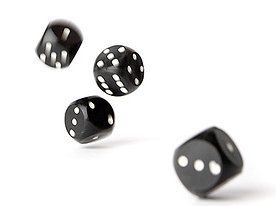
\includegraphics[height=0.25\textheight]{dices.png}
\includegraphics[height=0.25\textheight]{dna.png}
\end{center}
  \end{block}
}

\frame{ 
\frametitle{}
  \begin{block}{Examples: Binomial trials}
    \begin{itemize}
    \item Tossing a coin. $A$: Tails, $p = 1/2$
    \item Throwing a dice. $A$: Six, $p = 1/6$
    \item Child births
    \begin{itemize}
    \item $A$: Girl, $p = 0.5$
    \item $A$: Spina bifida (ryggmargsbrokk), $p = 0.001$
    \item $A$: Birth weight < 2500, $p = ?$
    \end{itemize}
  \item Epidemiology. $A$: Myocardial infarction, $p = ?$
  \item Genetics: both the mother and the father are carriers of the gene for
    cystic fibrosis. $A$: Child ill, $p = 1/4$
    \end{itemize}
  \end{block}
}

\frame{ 
\frametitle{}
  \begin{block}{Concepts}
    \begin{itemize}
    \item \hl{Counting variables}:
    \begin{itemize}
    \item How many times does event $A$ occur in a series of trials?
    \item Discrete variables (measured only by means of whole numbers)
    \end{itemize}
  \item \hl{Probability distributions
      for counting variables}: which is the probability for each
    possible number of events $A$?
    \end{itemize}
  \end{block}
}

\frame{ 
\frametitle{}
  \begin{block}{The probability for a certain sequence}
    \begin{itemize}
    \item Suppose that you carry out \hl{$\bm{n}$ trials}, looking
      \hl{for an event $\bm{A}$} to occur with
      \hl{probability $\bm{p}$} in each trial
    \item The result is a sequence like $A, \bar{A}, \bar{A}, A, \bar{A}, A,
      A, \bar{A}, ..., A$
    \item Now say that $A$ takes place $x$ times, meaning $n-x$
      occurrences of $\bar{A}$
    \item \hl{Which is the probability of such a sequence?}

    \pause

    \begin{itemize}
    \item Recall that probabilities for independent events may be
      multiplied!\\ P(sequence above) = $p(1-p)(1-p)p(1-p)pp(1-p) ...
      p$\vspace{1mm}
    \item $x$ number of $p$ and $n-x$ number of $(1-p)$:\\
      P(given sequence) = \hl{$p^x(1-p)^{n-x}$}
    \end{itemize}
    
    \pause
    
  \item But, you can get x successes out of n trials in \hl{many different
    orders}. What about the probability of $x$?
    
    \end{itemize}
  \end{block}
}

\frame{ 
\frametitle{}
  \begin{block}{The number of non-ordered selections}
    \begin{itemize}
    \item Want to find \hl{the number of ways that $\bm{x}$ objects can be
      chosen from a total of $\bm{n}$ objects}, regardless of order \pause
      \vspace{2mm}
     \item This number is given by \hl{the binomial coefficient $\binom{n}{x}$} \\ \pause
       \vspace{3mm} $\binom{n}{x} =
       \frac{n\cdot(n-1)\cdot(n-2)\cdot...\cdot(n-x+1)}{x!} =\frac{n!}{x!(n-x)!}$, where\vspace{4mm} \\
       $n\cdot(n-1)\cdot(n-2)\cdot...\cdot(n-x+1)$ is the number of
       ordered selections when picking $x$ objects out of a total of
       $n$ objects \\ \vspace{2mm}$x! =
       x\cdot(x-1)\cdot(x-2)\cdot...\cdot2\cdot1$ is the number of
       ways to order $x$ objects (or the number of permutations of $x$
       objects) \vspace{3mm}
       
     \item For example: $\binom{4}{3} = \frac{4\cdot 3\cdot
         2}{1\cdot 2\cdot 3} = 4$, and $\binom{10}{4} = \frac{10\cdot
         9\cdot 8\cdot 7}{1\cdot 2\cdot 3\cdot 4} = 420$

    \end{itemize}
  \end{block}
}

\frame{ 
\frametitle{}
  \begin{block}{Three ways to calculate the binomial coefficient $\binom{n}{x}$}
    \begin{itemize}
    \item Use the formula $\binom{n}{x} =
      \frac{n\cdot(n-1)\cdot(n-2)\cdot...\cdot(n-x+1)}{x!} =
      \frac{n!}{x!(n-x)!}$ \vspace{2mm} \\ where $n! =
      1\cdot2\cdot3\cdot ... \cdot (n-1) \cdot n$, and $0! = 1$  \vspace{3mm}\\ \pause
    \item Use a calculator or computer. Usually the notation is
      $\binom{n}{x} = nCx(n,x)$ \vspace{3mm}\\ \pause
    \item Use Pascal's triangle (see next slide)
    \end{itemize}
  \end{block}
}

\frame{
\frametitle{}
\begin{block}{Pascal's triangle}
  \begin{figure}[ht]
    \begin{center}
      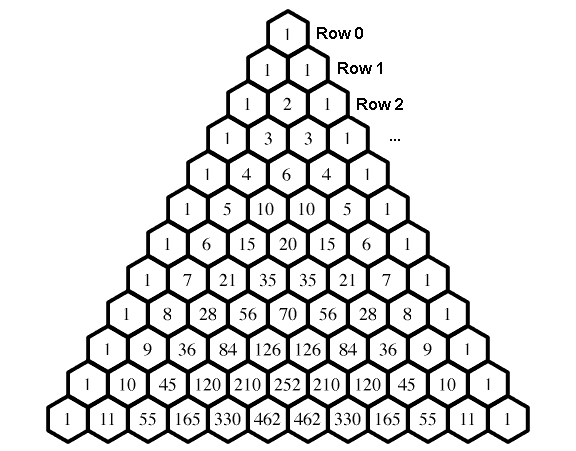
\includegraphics[height=0.5\textheight]{pascal.png}
      %\caption{}
    \end{center}
  \end{figure}

    \begin{itemize}
    \item $\binom{n}{x}$ refers to row $n$, place number $x+1$ from the left \pause
    \item It can be shown directly from the definition (formula) of
      the binomial coefficient that $\binom{n}{x} + \binom{n}{x+1} =
      \binom{n+1}{x+1}$
    \end{itemize}
\end{block}
}


\frame{ 
\frametitle{}
  \begin{block}{Summary of the last four slides...}
    We looked for an event $A$ with probability $p$ in $n$ trials and
    got a sequence $A, \bar{A}, \bar{A}, A ,\bar{A}, A, A, \bar{A}, ..., A$.
    
    In this sequence, $A$ took place $x$ times and $\bar{A}$ took
    place $(n-x)$ times.

  \begin{itemize}
  \item \hl{The probability of that particular sequence} was
    $p^x(1-p)^{n-x}$
  \item The sequence can be orded in many different ways, all with the
    same probability
  \item \hl{The number of ways to sort the sequence} is given by $\binom{n}{x}$
  \end{itemize}
  \vspace{3mm}
  We can now derive (or have already) the binomial distribution
  function, that is, the probability $P(x)$ for every possible $x$.
  \end{block}
}

\section{Binomial distribution}

\frame{ 
\frametitle{Binomial distribution}
  \begin{block}{Binomial probability distribution}
    \begin{itemize}
    \item We observe $n$ trials. The probability that $A$ occurs
      exactly $x$ times is given by\\ \vspace{3mm}

     \hl{ $P(X = x) = \binom{n}{x} p^x (1-p)^{n-x}$}, \\ \vspace{3mm}
      
     or \\ \vspace{3mm}
     
     $P(X = x) = $ \hl{the number of ways to
       distribute $\bm{x}$ events $\bm{A}$ in a sequence of length $\bm{n}$} $\bm{\times}$
     \hl{the probability of one particular
       sequence with $\bm{x}$ events $\bm{A}$}
       \end{itemize}
  \end{block}
}

\frame{
\frametitle{}
\begin{block}{Example: The binomial distribution for $n = 8$ and $p = 0.15$}
\hspace{5mm}  
\begin{figure}[ht]
    \begin{center}
      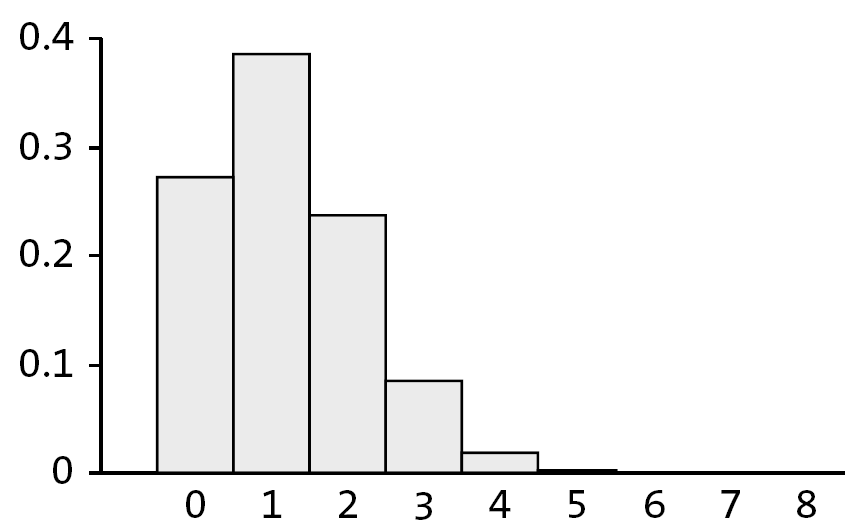
\includegraphics[height=0.55\textheight]{Figur4-2edited.png}
      %\caption{}
    \end{center}
  \end{figure}
       \begin{itemize}
       \item Often written Binomial(n=8, p=0.15), or Bin(8,0.15)
    \end{itemize}
\end{block}
}

\frame{ 
\frametitle{}
  \begin{block}{Properties of probability distributions in general}
       \begin{itemize}
       \item If you sum or integrate over all possible outcomes for a
         probability distribution, you should get 1
       \item Not surprising, from the probability theory lecture!
       \item Most probability distributions have an expected value
         (corresponding to the mean) and a variance (or standard
         deviation)
       \item For the binomial distribution: \\ $E(X) = np$ \\ $Var(X) =
         np(1-p)$
    \end{itemize}
  \end{block}
}

\frame{
\frametitle{}
\begin{block}{Example: binomial distribution for $n = 8$ and $p = 0.15$ (cont.)}
\hspace{5mm}  
\begin{figure}[ht]
    \begin{center}
      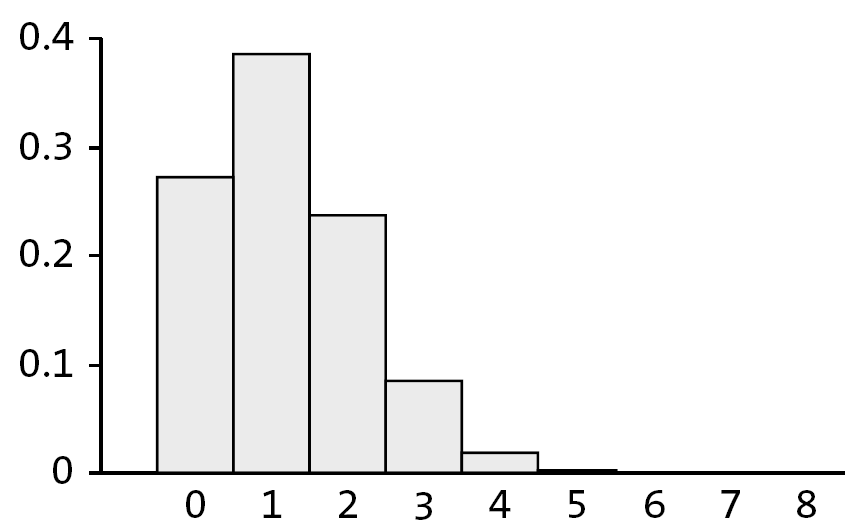
\includegraphics[height=0.40\textheight]{Figur4-2edited.png}
      %\caption{}
    \end{center}
  \end{figure}
  Let's say $p = 0.15$ is the probability that a person signing up to
  test for a certain disease get a positive result. A certain day you
  are going to do $n = 8$ such tests.
       \begin{itemize}
       \item What is the expected number of positive tests (the mean)?
       \item What is the variance and the standard deviation?
       \item What is the probability that you get 2 or more positives?
    \end{itemize}
\end{block}
}

\frame{
\frametitle{}
\begin{block}{Histograms from a binomial distribution with $n = 8$ trials, and four different values of $p$}
  \begin{figure}[ht]
    \begin{center}
      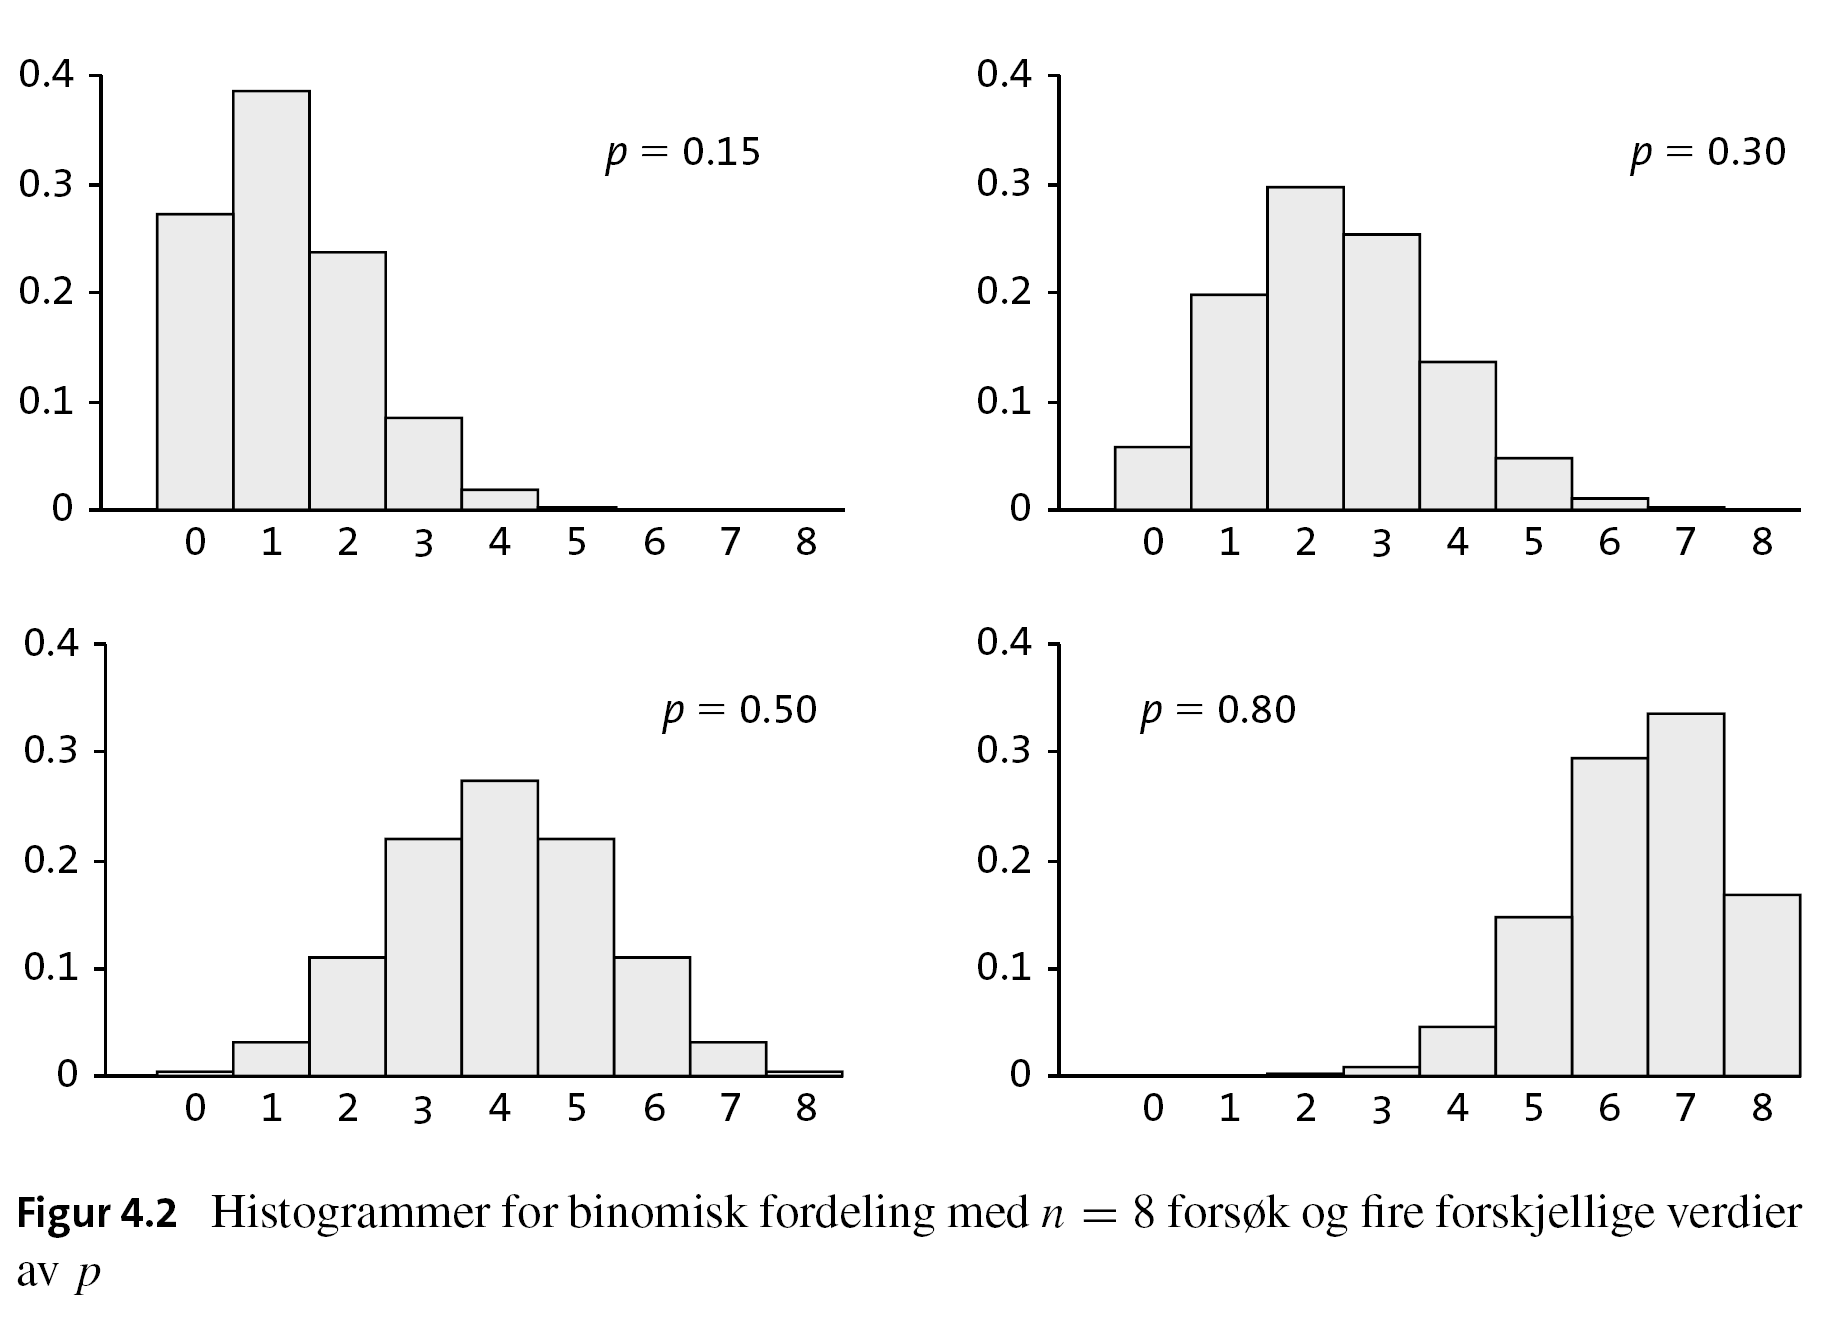
\includegraphics[height=0.75\textheight]{Figur4-2.png}
      %\caption{}
    \end{center}
  \end{figure}
\end{block}
}

\frame{ 
\frametitle{}
  \begin{block}{Example: Blood type (without using the formula)}
    Consider three randomly sampled individuals. How many have blood
    type A? \vspace{2mm}
    \begin{itemize}
    \item Independent individuals (random sampling)
    \item The only outcomes are \emph{bloodtype A} or \emph{not bloodtype A}
    \item Constant probabilities: $P(\text{A}) = 0.4$ and $P(\text{not
        A}) = 1-0.4 = 0.6$
    \end{itemize}
  \end{block}
}

\frame{ 
\frametitle{}
\begin{block}{}
All possible combinations for the three persons:
\begin{center}
\begin{tabular}{|c|c|c|c|}
\hline
Person 1 & Person 2 & Person 3 & Probability\\
\hline
A & A & A & $0.4\cdot 0.4 \cdot 0.4=0.064$\\
A & A & Not A & $0.4 \cdot 0.4 \cdot 0.6=0.096$\\
A & Not A & A & $0.4 \cdot 0.6 \cdot 0.4=0.096$\\
Not A & A & A & $0.6 \cdot 0.4 \cdot 0.4=0.096$\\
A & Not A & Not A & $0.4 \cdot 0.6 \cdot 0.6=0.144$\\
Not A & A & Not A & $0.6 \cdot 0.4 \cdot 0.6=0.144$\\
Not A & Not A & A & $0.6 \cdot 0.6 \cdot 0.4=0.144$\\
Not A & Not A & Not A & $0.6 \cdot 0.6 \cdot 0.6=0.216$\\
\hline
{} &  &  & $= 1$ \\
\hline
\end{tabular}
\end{center}
\end{block}
}

\frame{ 
\frametitle{}
\begin{block}{}
The binomial distribution for the number of people with blood
  type A is then: 
\begin{center}
\begin{tabular}{|c|c|}
\hline
Number of people & Probability\\
with blood type A & {} \\
\hline
0 & 0.216 \\
1 & $3 \cdot 0.144 = 0.432$ \\
2 & $3 \cdot 0.096 = 0.288$ \\
3 & 0.064 \\
\hline
{} & $= 1$ \\
\hline
\end{tabular}
\end{center}
\end{block}
}

\frame{ 
\frametitle{}
  \begin{block}{Example: Family with four kids}
    We're looking at a family with four kids, with no monozygotic
    twins, so the gender of the kids are (approx.) independent. The
    probability of getting a boy in Norway is 0.514. \vspace{2mm}
    \begin{itemize}
    \item What is the probability that two of the kids are boys? \\
      \vspace{2mm} $P(X=2) = \binom{4}{2} \cdot 0.514^2 \cdot 0.486^2$\\ \vspace{3mm}\hspace{1.55cm} $=
      \frac{4 \cdot 3}{2 \cdot 1} \cdot 0.514^2 \cdot 0.486^2 = 0.374$
    \end{itemize}
  \end{block}
}

\frame{
\frametitle{}
\begin{block}{}
    \begin{itemize}
    \item When the gender distribution of 7745 American families are
      given, together with the probability distribution from the
      binomial distribution we get this table:
    \end{itemize}
  \begin{figure}[ht]
    \begin{center}
      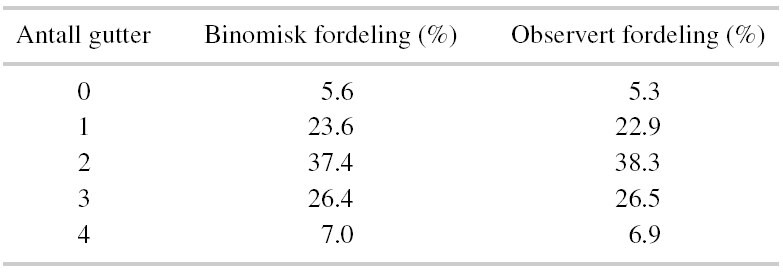
\includegraphics[width=0.75\textwidth]{tabells96.png}
      %\caption{}
    \end{center}
  \end{figure}
    \begin{itemize}
    \item We observe a good agreement!
    \end{itemize}
\end{block}
}

\frame{ 
\frametitle{}
  \begin{block}{Example: Multiple choice exam}
    Suppose a person knows absolutely nothing, and simply guesses on a
    12 item test with three alternatives.  What is their probability
    of passing the test, if 65\% is the passing mark?  \vspace{2mm}
    \begin{itemize}
    \item  You need 8 right to pass: 0.65 $\cdot$ 12 = 7.8
    \item 
      \vspace{2mm} $P(X = 8) = \binom{12}{8} \cdot 0.33^8 \cdot 0.66^{4} = 0.15$\\
      \vspace{2mm} $P(X = 9) = \binom{12}{9} \cdot 0.33^9 \cdot 0.66^{3} = 0.0033$\\
      \vspace{2mm} $P(X = 10) = \binom{12}{10} \cdot 0.33^{10} \cdot 0.66^{2} = 0.00050$\\
      \vspace{2mm} $P(X = 11) = \binom{12}{11} \cdot 0.33^{11} \cdot 0.66^{1} = 0.000045$\\
      \vspace{2mm} $P(X = 12) = \binom{12}{12} \cdot 0.33^{12} \cdot 0.66^{0} = 0.0000019$ \vspace{2mm}
    \item The probability to pass is $P(X \geq 8) \approx 0.15$
    \end{itemize}
  \end{block}
}

%\section{Introduction to hypothesis testing}
%
%\frame{ 
%\frametitle{Introduction to hypothesis testing}
%  \begin{block}{Statistical hypothesis testing}
%    \begin{itemize}
%    \item A method to \hl{draw conclusions from uncertain data}, estimating
%      the uncertainty in the conclusion
%    \item Based on the computation of a particular probability, called
%      the \hl{P value} (The probability for
%      the given result or a more extreme result to occur)
%    \end{itemize}
%  \end{block}
%  \begin{block}{}
%    We introduce hypothesis testing trough an example related to the
%    binomial distribution (\hl{the binomial
%      test}). More about Hypothesis testing in general tomorrow.
%  \end{block}
%}
%
%\frame{ 
%\frametitle{}
%  \begin{block}{Example: Clinical trial}
%    Want to try out a \hl{new medicine against migraine}. Let's denote the
%    new medicine $N$ and the traditional one $T$. Each patient get
%    $N$ one month, and $T$ another month. We want to find out which
%    month the patient feels the best/have less migraine. The trial is
%    \emph{randomized} and made \emph{blind} to make it fair. \vspace{1mm}
%  \end{block}
% \begin{itemize}
% \item \hl{Cross over study}: Eight patients try both medications in
%   randomized order
%    \end{itemize}
%}
%
%\frame{ 
%\frametitle{}
%  \begin{block}{}
%    \begin{itemize}
%    \item Say that 7 of totally 8 patients preferred $N$
%    \item Is $N$ better than $T$?
%    \item Let $p$ be the probability of a patient preferring $N$
%    \item Null hypothesis: $H_0: p = 1/2$ (Both treatments equally good)
%    \item Alternative hypothesis: $H_A: p > 1/2$ ($N$ is better)
%    \end{itemize}
%  \end{block}
%}
%
%\frame{ 
%\frametitle{}
%  \begin{block}{}
%    \begin{itemize}
%    \item If the null hypothesis holds, $X$ is binomially distributed with $n = 8$ and $p = 1/2$
%    \item P value: \\ \vspace{2mm}
%      
%      $P(X \geq 7 | H_0) = \binom{8}{7} \cdot (1/2)^7 \cdot (1/2)^1 +
%      \binom{8}{8} \cdot (1/2)^8 \cdot (1/2)^0$\\ \vspace{2mm} \hspace{2.1cm} $= 0.035 = 3.5\%$
%
%      \vspace{2mm}
%
%    \item Mindset: If P is small, this indicates that $H_0$ is not likely to be true
%    \item We reject $H_0$ and accept $H_A$ if $P$ is smaller than the
%      \hl{level of significance}. This is
%      often set to $5\%$, or sometimes $1\%$ or less
%    \item With a $5\%$ level of significance we would reject $H_0$
%      and say that $N$ is a better drug than $T$
%    \end{itemize}
%  \end{block}
%}

%% \frame{
%% \frametitle{}
%% \begin{block}{}
%%   \begin{figure}[ht]
%%     \begin{center}
%%       \includegraphics[height=0.82\textheight]{Figur4-1.png}
%%       %\caption{}
%%     \end{center}
%%   \end{figure}
%% \end{block}
%% }

\section{Summary}

\frame{ 
\frametitle{Summary}
  \begin{block}{Key words}
    \begin{itemize}
    \item (Discrete) Probability distributions
    \item Binomial trials
    \item Counting variables
    \item The binomial coefficient
    \item The binomial distribution
    \end{itemize}
  \end{block}
  \begin{block}{Notation}
    \begin{itemize}
    \item $x!$
    \item $\binom{n}{x}$
    \item $P(X = x)$
    \end{itemize}
  \end{block}
}

\end{document}

